\chapter{Stopped flow \SOtwo measurements}\label{ch:stoppedflow}

As a first step in this research, experiments on blood using a stopped flow setup were completed, using a similar protocol and design used in previous work by the group.
Stopped flow measurements are the typical method used in the literature for these blood oxygenation \Ttwo experiments, and there a number of examples in the literature\cite{BrooksComparisont2relaxation1995,BryantMagneticrelaxationblood1990,GomoriNMRRelaxationTimes1987} (although as mentioned in the introduction, relatively few at low field.
These experiments used the stopped flow experimental setup from \autoref{ch:exptsetup}, with 3 different magnet systems at different fields to observe changes in \Ttwo at a number of levels of oxygenation.
These also provide a benchmark for the continuous flow setup, as it removes any effects which occur because of flow.

\section{Experimental Protocol}
For this series of experiments, measurements of \Ttwo were made at a series of oxygenation steps, which we attempted to set by adjusting the gas mix going into the oxygenator.
These steps are shown graphically in \autoref{fig:sf-protocol}
After the flow circuit was assembled, the blood sample was loaded into the tubes and oxygenator, using the standard connectors on the bag.
The pump was switched on, and gas at 21\% \Otwo was flowed through to bring the oxygenation and temperature of the blood up to the 100\% starting point for the experiments.
The blood was allowed to flow through the circuit for a period of time to allow the temperature to stabilise, before an initial test with the iStat.
During this time, the probes were tuned and matched, and pulse sequence parameters such as pulse power and \textit{B\textsubscript{1}} frequency were calibrated (using FIDs on the Halbach system, and CPMG detection on the MOLE.)
\begin{figure}[t]
\centering
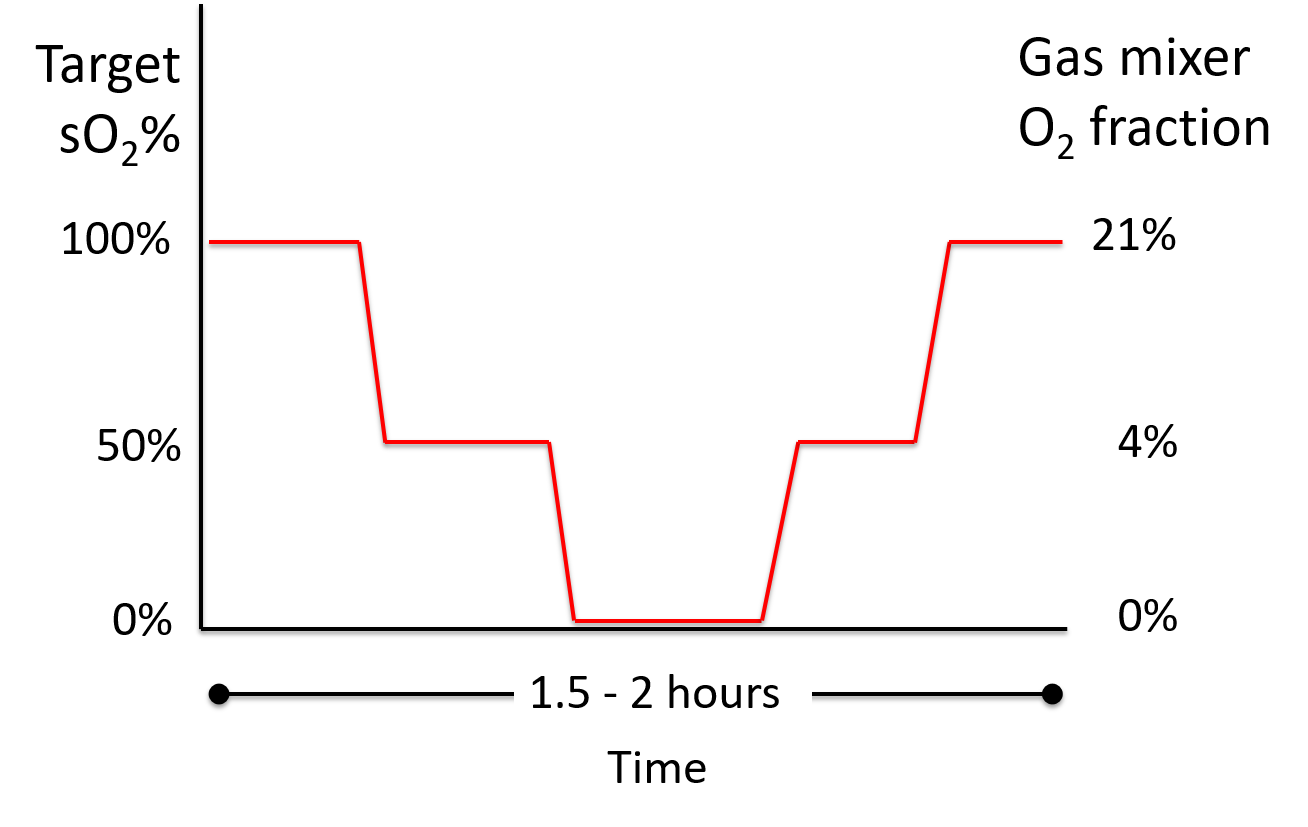
\includegraphics[width=0.7\textwidth]{figures/stoppedflow/stoppedflowprotocol.png}
\caption{Outline of experimental protocol for stopped flow experiments}
\label{fig:sf-protocol}
\end{figure}

If this showed that the pH, \SOtwo and HcT were normal, the flow was stopped and measurements on the two in-line NMR systems were started.
If the blood pH was significantly below 7, it was adjusted by adding sodium bicarbonate solution.
Typically \TR = \SI{2.1}{s}, with echo times of \SIlist{0.25;0.5;1;5}{ms} on the Halbach, and \SIlist{0.25; 0.5; 1}{ms} on the MOLE (these were limited by the magnetic field gradients in each system).
The number of echoes was adjusted to create an echo train \SI{600}{ms} long.
4 scans with phase cycling were used on the Halbach, but the poorer signal to noise on the MOLE meant that 16 scans were required.
Once these measurements had completed, the pump was turned on briefly to agitate the blood and minimize any effects of settling before repeating the NMR measurements.
A \SI{2}{ml} sample of blood in the circuit was also syringed into a clean \SI{5}{mm} NMR tube for the Spinsolve measurements.
These tubes were sealed with the caps provided by the manufacturer.
On the Spinsolve, typical experimental parameters were \TR = \SI{20}{s} with a 4 scan phase cycle, and with 4 echo times: \SIlist{0.5;2.5;5;10}{ms}.
Again, the number of echoes was set to give an echo train with a fixed length of \SI{10}{s}.

\begin{figure}[t]
\centering
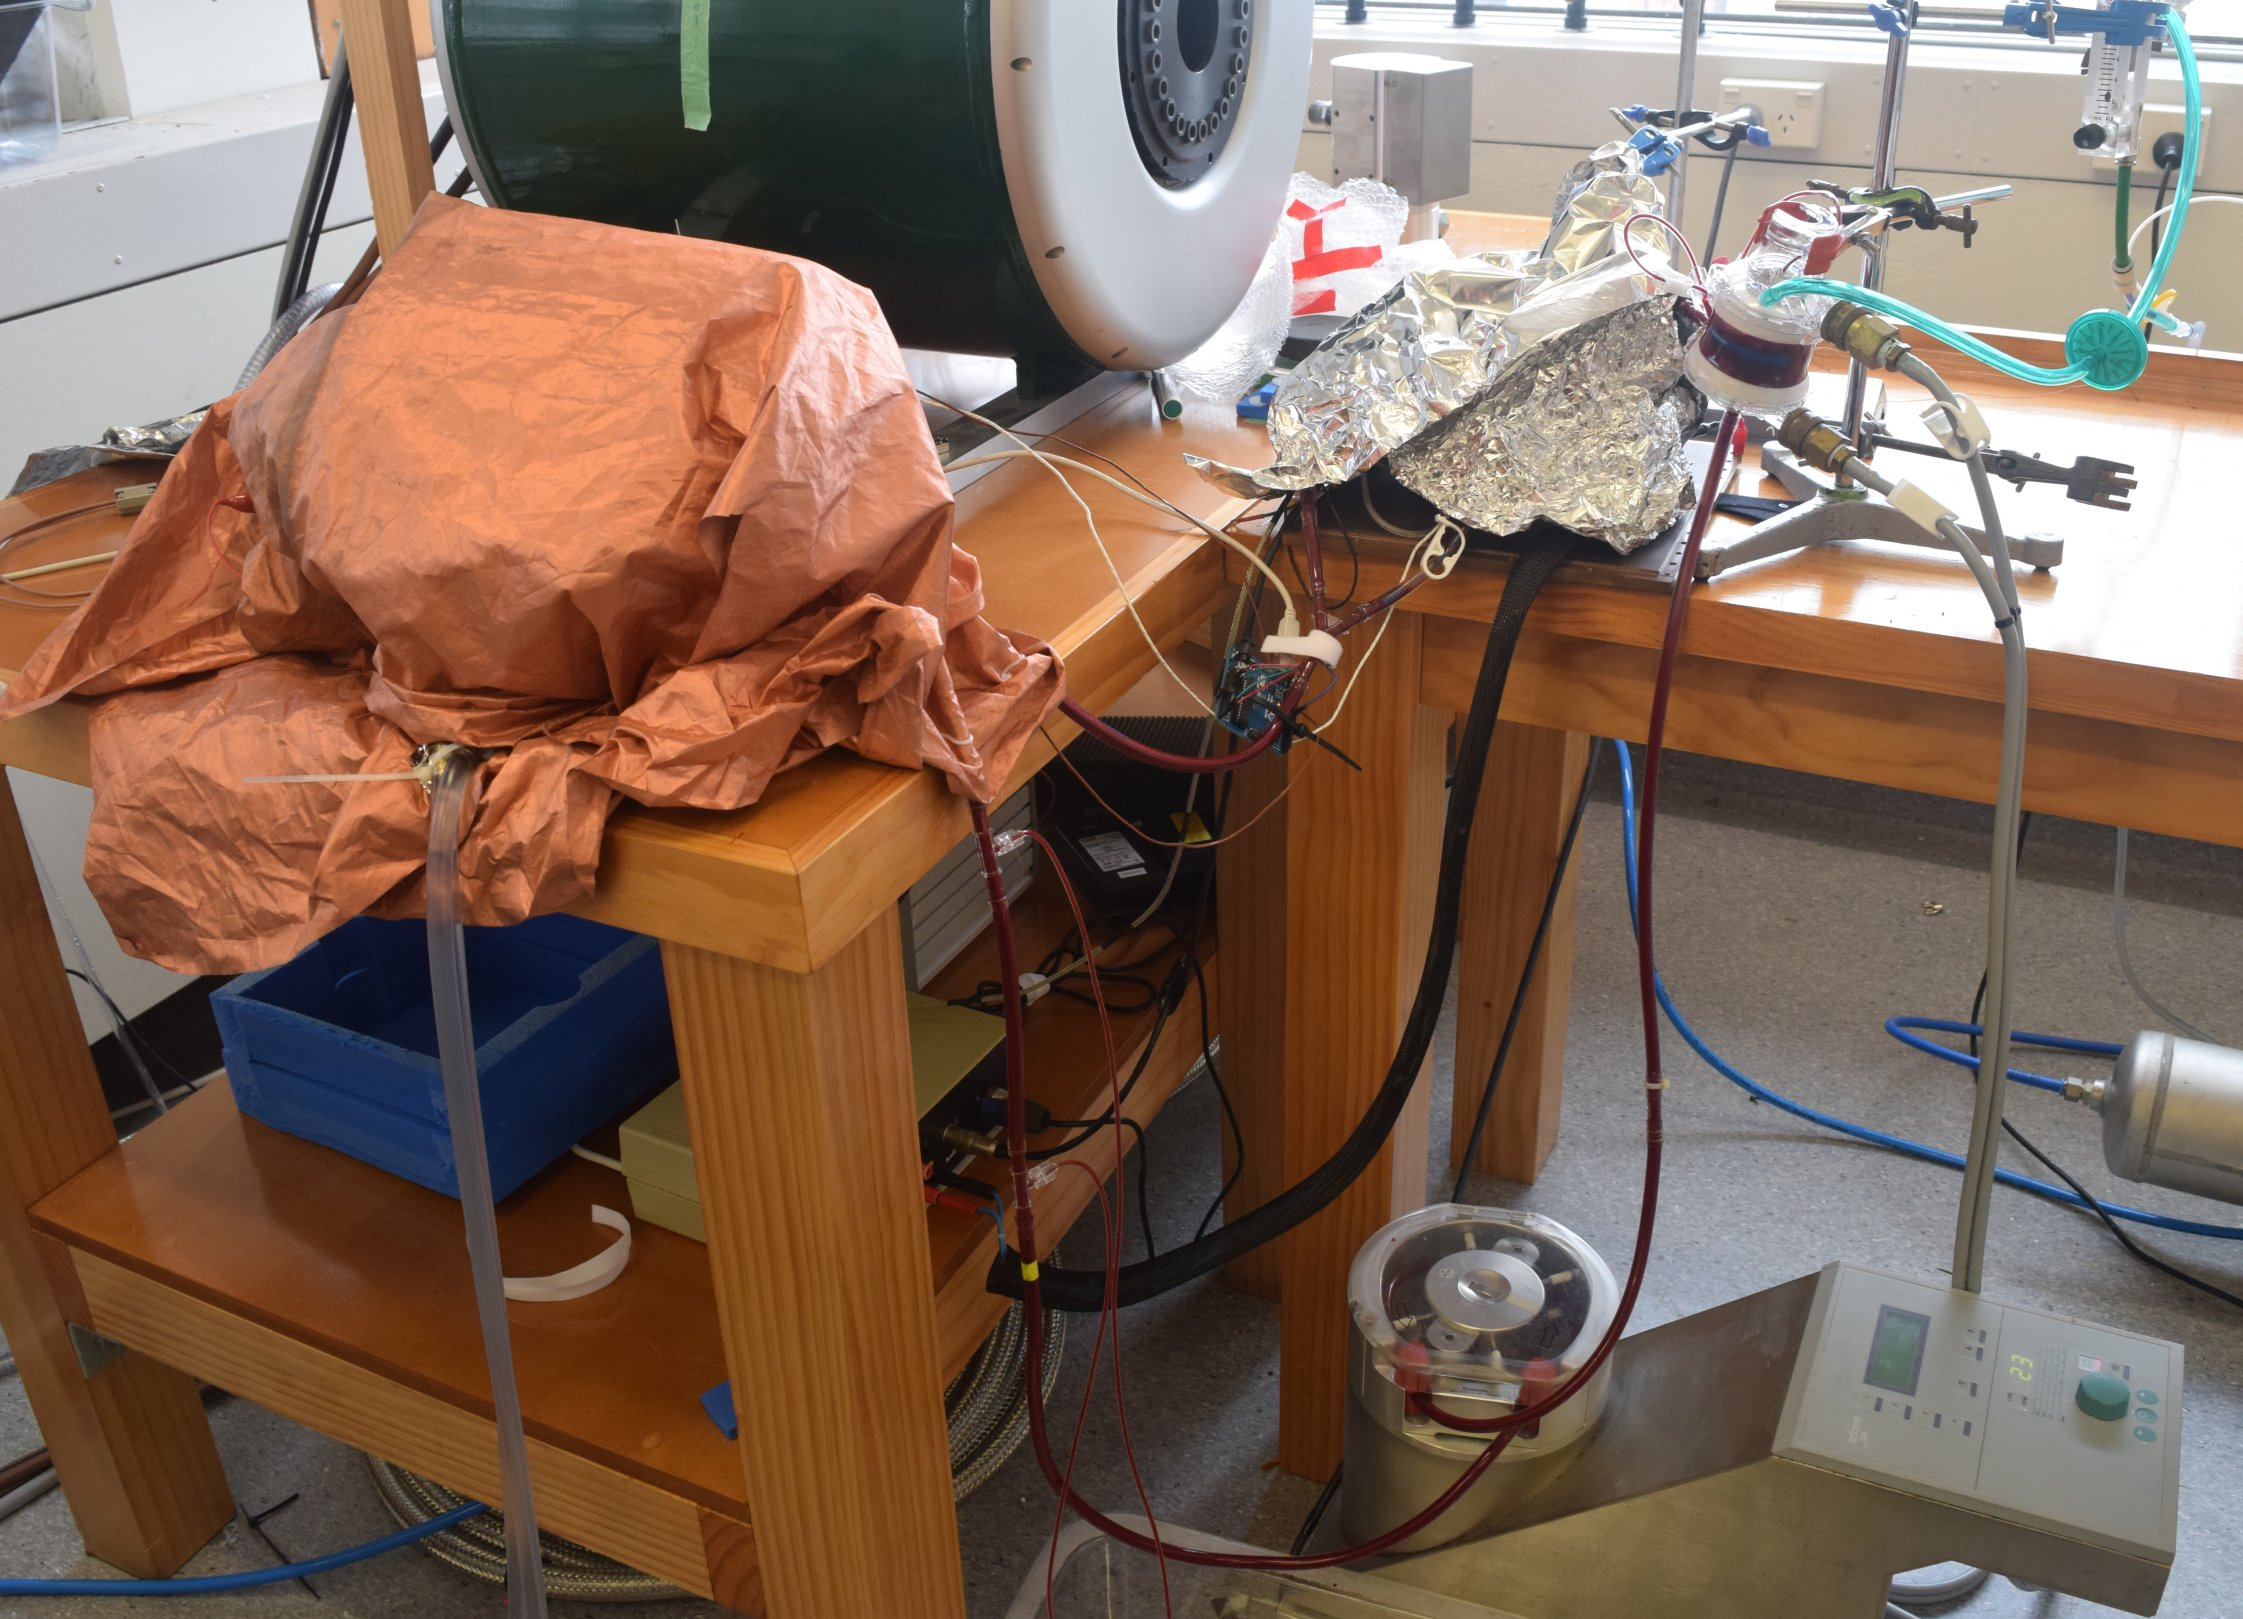
\includegraphics[width=0.8\textwidth]{figures/stoppedflow/stoppedflowsetup.jpg}
\caption{Experimental setup for stopped flow experiments (gas mixer and analyser not shown)}
\label{fig:sf-stoppedflowsetup}
\end{figure}

The \SOtwo was then lowered to an intermediate value (around 50\%).
Flow was turned back on and the gas mix set to 5\% \Otwo, which we had found produced these levels of oxygenation.
After waiting for the \SOtwo to reach the desired level, a sample of blood was taken from the flow circuit and the iStat was used to confirm the \SOtwo.
The flow was stopped, two sets of NMR measurements were completed as above, and a sample was removed for the Spinsolve.

This process was repeated again to measure \Ttwo at a very low oxygenation (10\% or less), by setting the gas mix to 0\% \Otwo.
Afterwards, these steps were reversed to increase the oxygenation again, taking a measurement at an intermediate value of \SOtwo on the way up as well.

Data was extracted and processed using Python, in JuPyter notebooks.
Each echo train is phased, and each echo is summed to give a single value for the signal at each echo time.
The resulting decay is fit to a monoexponential decay using non-linear least squares fitting, which results in a single \Ttwo value at each \SOtwo.

\section{Results}
\subsection{Spinsolve results}
Two examples of the CPMG decays measured on the Spinsolve are shown in \autoref{fig:sf-spinsolveCPMG}.
Plotting the log of the echo amplitudes against time gives a straight line, which indicates that the decay is mono-exponential.
This agrees with what is reported in the literature.

This data also shows even-echo rephasing occuring in the decays measured with long echo times (in red).
Where this was visible, only the even echoes were used in the curve fitting routine to find \Ttwo.

%Graph generated in processBloodOxygenation1/Spinsolve data 170728
\begin{figure}[ht]
\centering

\begin{subfigure}[t]{0.48\textwidth}
\caption{\SOtwo = 95\%}
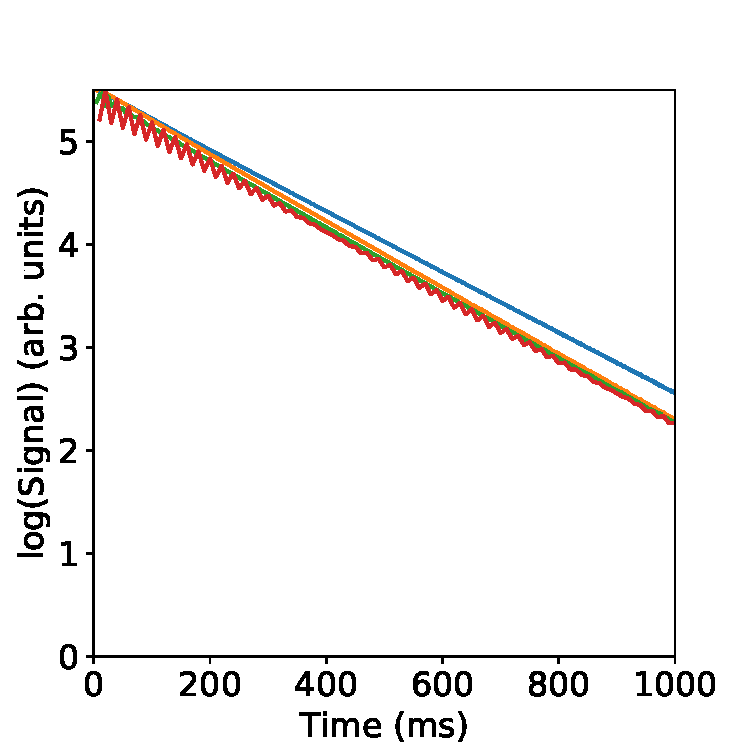
\includegraphics[width=\textwidth]{figures/stoppedflow/spinsolveCPMG95.pdf}
\end{subfigure}
\begin{subfigure}[t]{0.48\textwidth}
\caption{\SOtwo = 9\%}
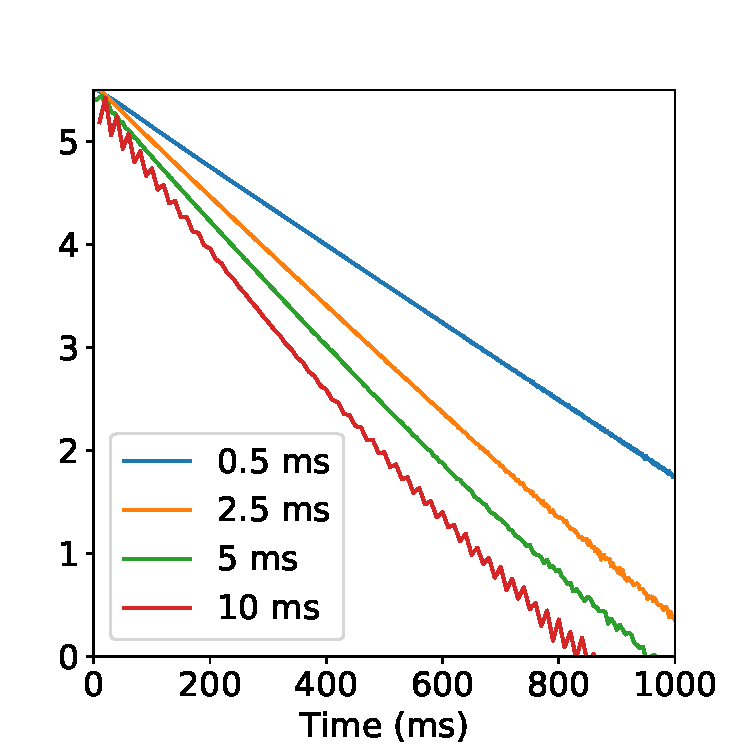
\includegraphics[width=\textwidth]{figures/stoppedflow/spinsolveCPMG9.pdf}
\end{subfigure}

\caption{Examples of CPMG decays measured on the Spinsolve for oxygenated and deoxygenated blood}
\label{fig:sf-spinsolveCPMG}
\end{figure}

Decays were measured at a range of oxygenations and fitted to obtain \Ttwo.
These results are shown in \autoref{fig:sf-spinsolveT2SO2}.

%Graph generated in processBloodOxygenation1/Spinsolve data 170728
\begin{figure}[ht]
\centering
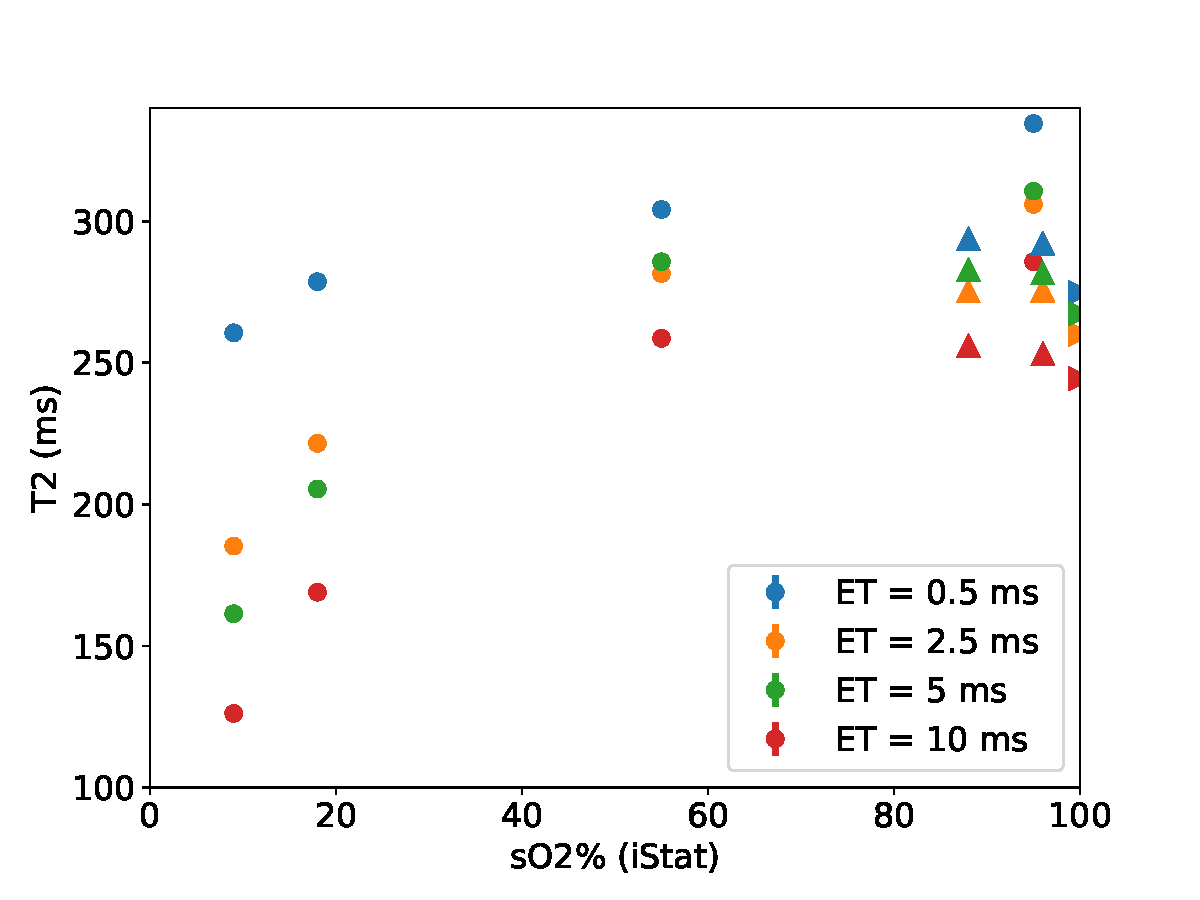
\includegraphics[width=\textwidth]{figures/stoppedflow/spinsolveT2SO2down.pdf}
\caption[\Ttwo vs. \SOtwo measured on the Spinsolve]{\Ttwo at different levels of oxygenation, measured on the Spinsolve. Circles indicate samples measured when deoxygenating the blood, while upwards pointing triangles are samples when oxygenating it (see experimental protocol). Right pointing triangles are a sample hyperoxygenated with 30\% \Otwo}
\label{fig:sf-spinsolveT2SO2}
\end{figure}

As the oxygenation of the blood was lowered, the \Ttwo decreases from \SI{334}{ms} to \SI{260}{ms} at the short echo time, while changes more drastically from \SI{285}{ms} to \SI{126}{ms} at the longest echo time.
This shows that the changes in oxygenation are visible in this \SI{1}{T} system.
The shorter \Ttwo at long echo time is expected, as there is more time for dephasing to occur, as discussed in \autoref{sec:back-T2SO2}.
The separation between the short echo time and long echo time \Ttwo{}s also increases at lower \SOtwo.
This is predicted by theory, as the susceptibility difference and induced field inhomogeneity is increased with high levels of deoxy-haemoglobin.

One difficulty we had was recovering the original \Ttwo value when the blood was re-oxygenated.
This is shown by the two samples measured while oxygenating (triangles in \autoref{fig:sf-spinsolveT2SO2}.
A number of experiments were conducted to investigate the cause of this, and these are discussed below.

\subsection{Halbach results}
%Graph produced in Halbach 170726
\begin{figure}[h]
\centering
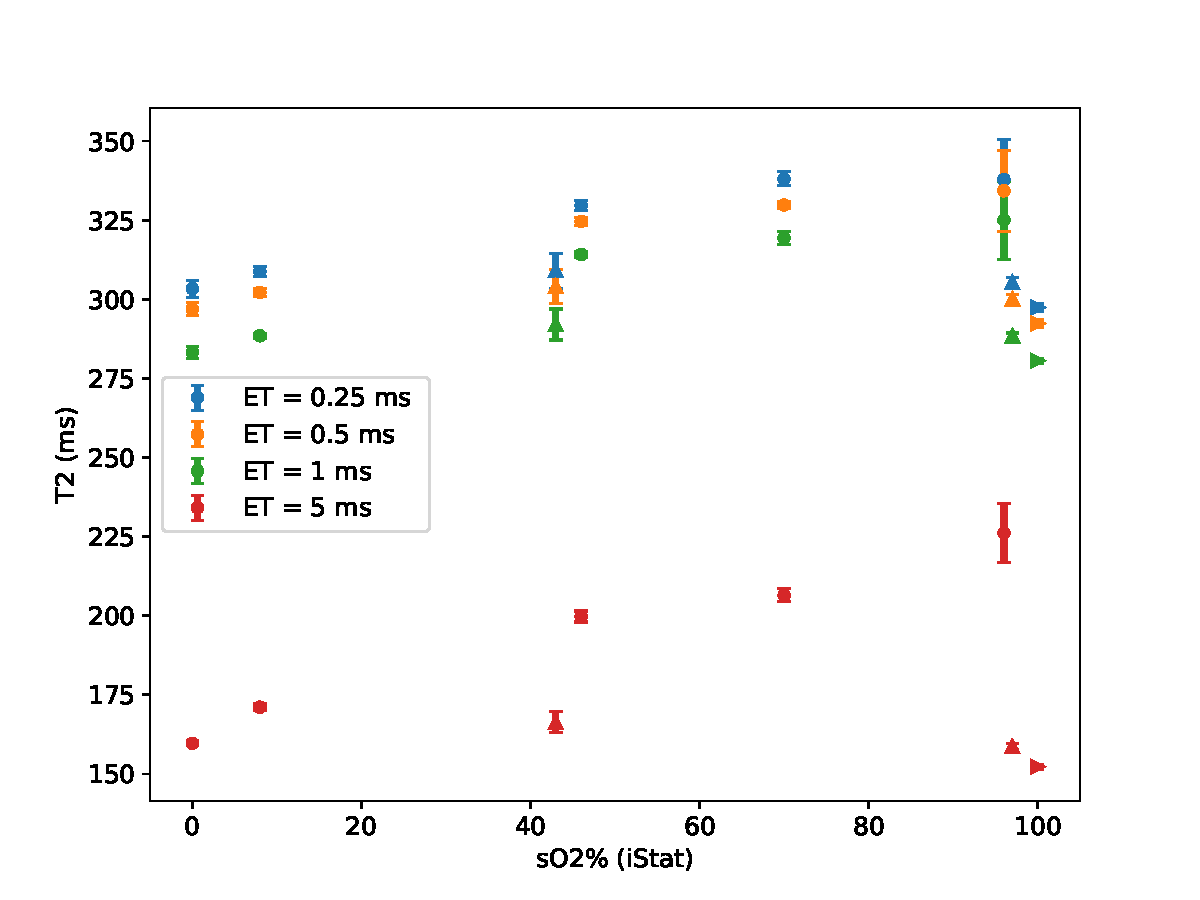
\includegraphics[width=\textwidth]{figures/stoppedflow/halbachT2SO2.pdf}
\caption[Stopped flow \Ttwo vs. \SOtwo measured on the Halbach system]{\Ttwo vs. \SOtwo measured on the Halbach system. Circles indicate samples measured when deoxygenating, upwards triangles are measured when oxygenating and right-pointing triangles are a sample oxygenated with 30\% \Otwo. Error bars represent standard error (n=3)}
\label{fig:sf-halbachT2SO2}
\end{figure}

The Halbach magnet system was run inline with the flow circuit, making it easier to measure more data points.
As with the Spinsolve results, the CPMG decays were found to be monoexponential, however there was no appearance of even echo rephasing in the CPMG decays.
In this experiment, the deoxygenation causes the \Ttwo to decrease from \SI{337}{ms} to \SI{303}{ms} for the short echo time, and from \SI{226}{ms} to \SI{152}{ms} for the \SI{5}{ms} echo time.
The strong field gradients in this system means that the CPMG experiments are sensitive to the diffusion of protons moving through the gradient, which causes longer echo times to measure a shorter \Ttwo.
This can be seen in the position of the \SI{5}{ms} points (red), which are significantly lower than points at \SI{<1}{ms}.
In this experiment, measurements were also completed with echo times of \SIlist{8;12}{ms}, but these did not show any trends due to the strong relaxation from the field inhomogeneities.

Like in the Spinsolve experiments, the \Ttwo values in this experiment did not return to the same levels they did at the start of the experiment after reoxygenating, which suggests that this change is not solely related to the sampling method and storage of the Spinsolve samples.
The decrease from the initial \Ttwo measurement to the reoxygenated measurement appears to be approximately the same size (\SI{40}{ms}), although the decrease at the \SI{5}{ms} echo time is much greater.
This may also be related to problems with the Halbach magnet and probe, for example, changes in magnet temperature over the experiment time or slight movements or rotations of the probe inside the magnet, which would alter the gradients seen be the sample.

\subsection{MOLE results}
%Graph from Mole 170728
\begin{figure}[h]
\centering
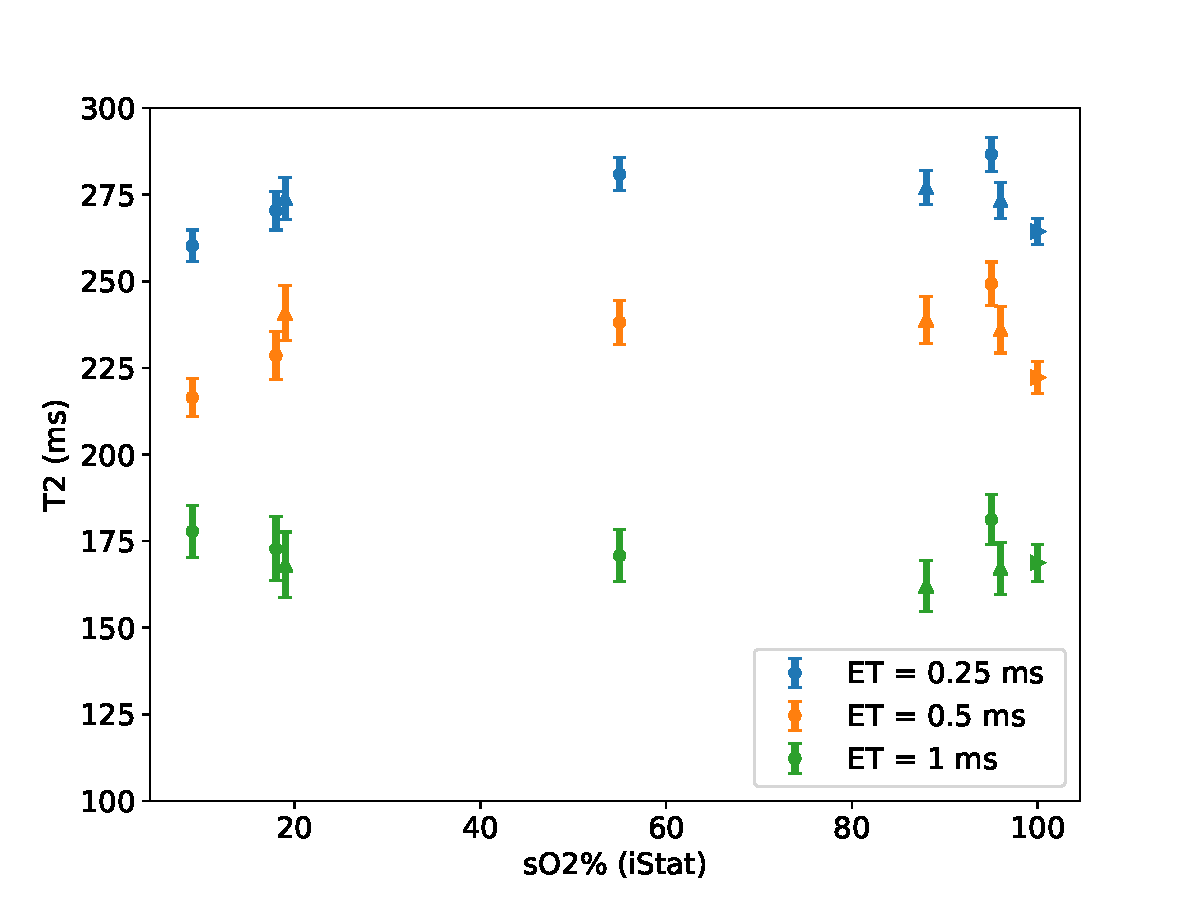
\includegraphics[width=\textwidth]{figures/stoppedflow/moleT2SO2.pdf}
\caption[Stopped flow \Ttwo vs. \SOtwo measured on the MOLE system]{\Ttwo vs. \SOtwo measured on the MOLE system. Circles indicate samples measured when deoxygenating, upwards triangles are measured when oxygenating and right-pointing triangles are a sample oxygenated with 30\% \Otwo. Error bars represent standard error (n=3)}
\label{fig:sf-moleT2SO2}
\end{figure}
%
Measurements on the MOLE had a significantly lower signal to noise than the other two systems.
This is related to both the reduced field strength (\SI{0.1}{T}), and the single-sided design of the magnet system.
Because of this, measurements took longer to acquire than on the other systems and the largest source of experimental uncertainty was from noise in the fitting process.

As expected, the change in \Ttwo as oxygenation was decreased was smaller again than in the higher field Spinsolve and Halbach system measurements.
At the \SI{0.25}{ms} echo time, the decrease from oxygenated to deoxygenated is \SI{25}{ms}, but at the \SI{1}{ns} echo time, the decrease is only \SI{5}{ms} (which is within experimental uncertainty.)
Additionally, the field inhomogeneity of the MOLE means that there is a significant decrease in the measured \Ttwo due to diffusion through the gradients of the magnet system.
Along with the decrease in the stregnth of the effect at this field, this could explain why there is little to no change at the \SI{1}{ms} echo time.

These results also show that \Ttwo is lower after reoxygenating, with a decrease of approximately \SI{15}{ms} between the initial \Ttwo and the \Ttwo after reoxygenation.
It is unlikely to be due to changes in the magnetic field gradients as the MOLE temperature is very well controlled, and the sample was the entire blood bag, which is larger than the sweet spot of the magnet.

\subsection{Field comparison}
Results for the different fields are combined in \autoref{fig:sf-fieldcomparison}, after converting the \Ttwo values for oxygenated and deoxygeneated blood into \Rtwo.
Although the data from the MOLE is strongly affected by its inhomogeneous field, taking the difference of the oxygenated and deoxygenated \Rtwo{}s should cancel this effect.

%Graph from Spinsolve 170728
\begin{figure}[h]
\centering
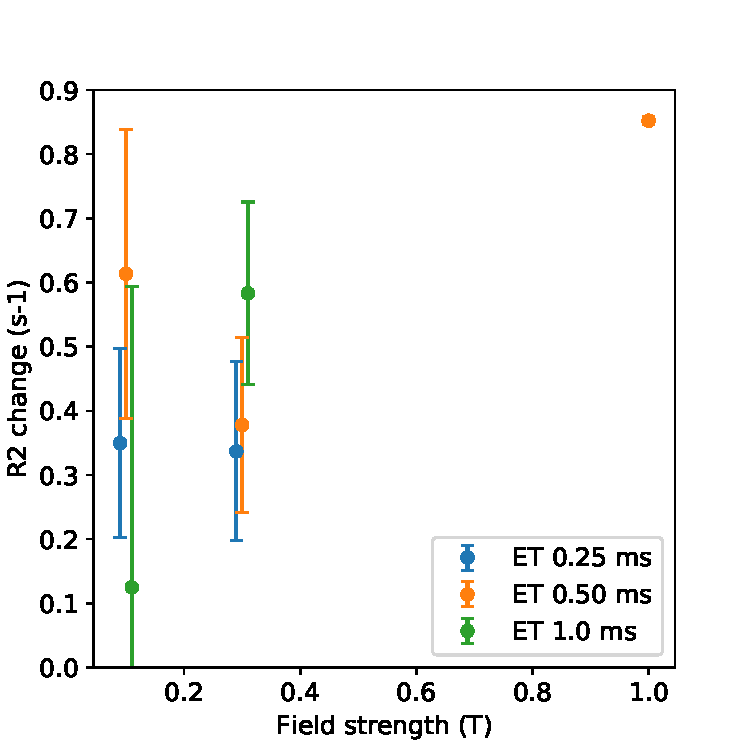
\includegraphics[width=0.8\textwidth]{figures/stoppedflow/fieldcomparison.pdf}
\caption[Change in \Rtwo for the three stopped flow systems]{Change in \Rtwo for the three stopped flow systems. Data points show \Rtwo\textsubscript{\textit{deoxy}} -- \Rtwo\textsubscript{\textit{oxy}} to remove the effect of background gradients. Note points are moved on the x-axis to allow comparison}
\label{fig:sf-fieldcomparison}
\end{figure}

\autoref{fig:sf-fieldcomparison} shows that the \Ttwo decrease is much larger at \SI{1}{T}, although data was only collected at the \SI{0.5}{ms}.
Additionally, the \SI{0.1}{\tesla} measurement shows that the change in \Rtwo is higher or the same as than the data point at \SI{0.3}{T}, which does not agree with the quadratic dependence from theory, however, the uncertainty in the MOLE data points is much larger.

%It is also possible that the exchange/diffusion theory is not as effective at these short echo times, and other processes are occuring, this might be discussed below TODO!!!!

\section{Discussions}

These results confirm that \Ttwo when decreasing \SOtwo occur at low fields, in agreement with the literature.
As noted in the introduction however, there are relatively few examples in the literature to compare them to.
Brooks et al. studied the field dependence of the \Ttwo decrease for oxygenated and deoxygenated blood, and found that the size of the \Rtwo change scales with \Bzero  squared\cite[Fig.1]{BrooksComparisont2relaxation1995}.
For their study however, they used a more conventional \SI{4}{ms} echo time, which makes the \Rtwo change from oxygenated to deoxygenated much larger (on the order of \SI{4}{s^{-1}} at \SI{0.5}{T}.)
This means that their results are not directly comparable with the results in \autoref{fig:sf-fieldcomparison}, where the echo time is less than \SI{1}{ms}.

We also encountered trouble with recovering the intial \Ttwo when reoxygenating the blood.
This was visible in all results above, where at high \SOtwo{}s, the reoxygenated \Ttwo values (upwards triangles)  are typically lower than the initial values (circles) by \SIrange{10}{40}{ms}.
In this set of experiments, several hypotheses were tested to investigate the cause of this.
The fact that it occured across all three systems (including the Spinsolve, which was used not part of the circuit) suggests that it is due to a physical change in the blood and not only related to changes in the flow circuit (although movement of the Halbach probe could not be ruled out.)

One possibility was that the blood was not completely reoxygenated, which could occur if the blood was damaged during storage or or the time at extremely low \SOtwo, and caused the \SOtwo measurement on the iStat to be inaccurate.
To test this, samples were hyper-oxygenated with 30\% \Otwo (rather than 21\%).
This caused an increase in the p\Otwo from \SIrange{110}{150}{mmHg} in the normally reoxygenated blood to \SIrange{180}{200}{mmHg} in the hyperoxygenated blood, and should have caused more of the remaining deoxy-haemoglobin to become oxy-haemoglobin, raising the \Ttwo.
Interestingly, we observed a further decrease in \Ttwo in all cases, shown by the right-triangles in the results.
This is not likely to be due to the paramagnetic effect of dissolved Oxygen, as this should have an extremely small effect on the \Ttwo at these relatively low p\Otwo values.
Ma et al. found that dissolved Oxygen in blood plasma causes \Rtwo to increase by \SI{2.3e-4}{s^{-1}\per\mmHg}~\cite{Maeffectdissolvedoxygen2016}, which would correspond to a change of \SI{0.04}{s^{-1}} at \SI{200}{mmHg}.

Another possibility was that a property of the blood had changed in the circuit, with some parameter that affects \Ttwo being different, for example the haematocrit increasing due to separation of plasma and red blood cells in the blood bag.
However, testing with the iStat showed that there were not significant changes to the parameters it measured between the start and end of the experiments.

Instead, we investigated whether red blood cells were being damaged by flowing through the circuit, and that this damage caused a decrease in \Ttwo.
This would explain the \Ttwo decrease after hyperoxygenation, which would be caused by spending more time in the flow circuit.
To test this, samples of the blood were removed from the circuit before and after the experiment.
These were centrifuged to separate the red blood cells and plasma, and the colour of the plasma was compared to identify whether significant haemolysis had occured.
An example of one test is included in \autoref{fig:sf-bloodbeforeafter}.
This effect was studied more quantitatively when it occured in the continuous flow experiments described in \autoref{ch:cont}.

\begin{figure}[t]
\centering
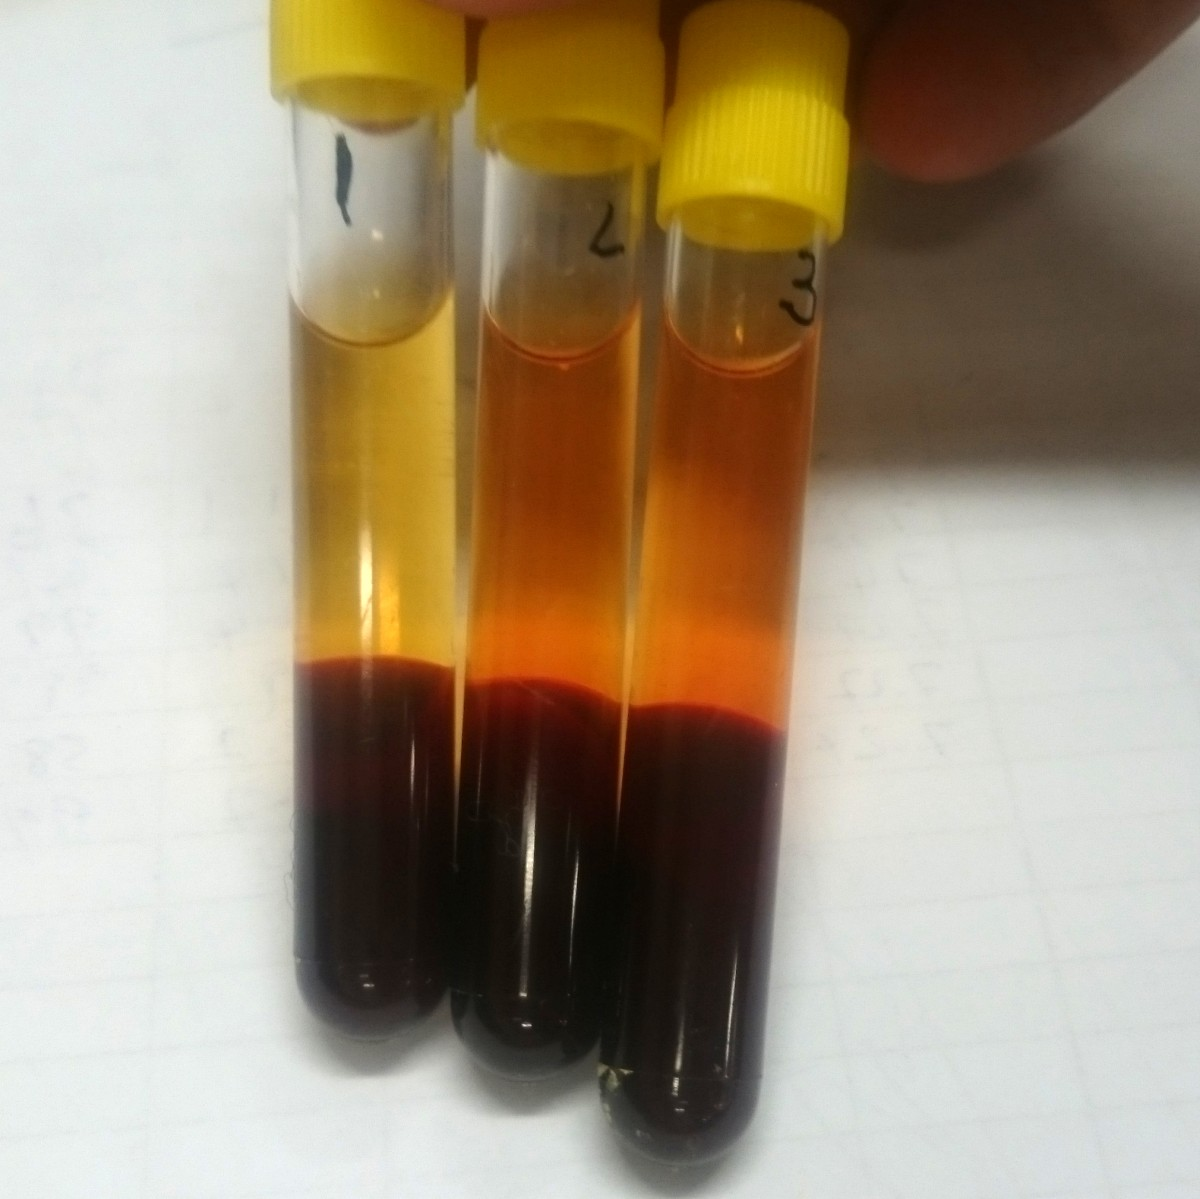
\includegraphics[width=0.5\textwidth]{figures/stoppedflow/samplecheck.jpg}
\caption[Centrifuged blood samples from start and end of experiment]{Centrifuged blood samples from before (tube 1, left), during (tube 2), and after stopped flow experiments (tube 3, right). Note the redder colour from the tubes on the right}
\label{fig:sf-bloodbeforeafter}
\end{figure}

While these results confirm that changes in \SOtwo can be observed at low field, there were some difficulties with this method of collecting data.
As the stopped flow system requires the flow to be stopped, it is possible that the blood could be changing within the scan time due to factors such as temperature dropping, or red blood cells separating from the plasma.
It was also very difficult to be able to `hit' desired intermediate values of oxygenation.
This is because of haemoglobin's strong affinity for Oxygen, which creates the very steep curve shown in \autoref{fig:back-po2so2}.
To be able to reach a specific intermediate levels of oxygenation would require more precision and stability in the gas mix output than were possible with this experimental setup.
Therefore, the continuous flow setup discussed in \autoref{sec:exptsetup-contflow} was designed for the next set of experiments.
Because the introduction of flow complicates everything, these stopped flow results are used as a benchmark for the continuous flow experiments.
